% \subsection{BigGAN}
In the BigGAN model (Figure~\ref{appendix_resblock_figure}), we use the ResNet \citep{he2016resnets} GAN architecture of \citep{zhang2018sagan}, which is identical to that used by \citep{miyato2018spectral}, but with the channel pattern in \discr{} modified so that the number of filters in the first convolutional layer of each block is equal to the number of output filters (rather than the number of input filters, as in \citet{miyato2018spectral, gulrajani2017improved}). 
We use a single shared class embedding in \gen{}, and skip connections for the latent vector $z$ (skip-$z$). In particular, we employ hierarchical latent spaces, so that the latent vector $z$ is split along its channel dimension into chunks of equal size ($20$-D in our case), and each chunk is concatenated to the shared class embedding and passed to a corresponding residual block as a conditioning vector.
The conditioning of each block is linearly projected to produce per-sample gains and biases for the BatchNorm layers of the block. The bias projections are zero-centered, while the gain projections are centered at $1$. Since the number of residual blocks depends on the image resolution, the full dimensionality of $z$ is 120 for $128\times 128$, 140 for $256\times 256$, and 160 for $512\times 512$ images.

The BigGAN-deep model (Figure~\ref{appendix_resblock_figure_deep}) differs from BigGAN in several aspects.
It uses a simpler variant of skip-$z$ conditioning: instead of first splitting $z$ into chunks, we concatenate the entire $z$ with the class embedding, and pass the resulting vector to each residual block through skip connections.
BigGAN-deep is based on residual blocks with bottlenecks~\citep{he2016resnets}, which incorporate two additional $1 \times 1$ convolutions: the first reduces the number of channels by a factor of $4$ before the more expensive $3 \times 3$ convolutions; the second produces the required number of output channels. 
While BigGAN relies on $1\times 1$ convolutions in the skip connections whenever the number of channels needs to change, in BigGAN-deep we use a different strategy aimed at preserving identity throughout the skip connections. In $\gen{}$, where the number of channels needs to be reduced, we simply retain the first group of channels and drop the rest to produce the required number of channels. In $\discr{}$, where the number of channels should be increased, we pass the input channels unperturbed, and concatenate them with the remaining channels produced by a $1 \times 1$ convolution.
As far as the network configuration is concerned, the discriminator is an exact reflection of the generator. There are two blocks at each resolution (BigGAN uses one), and as a result BigGAN-deep is four times deeper than BigGAN. 
Despite their increased depth, the BigGAN-deep models have significantly fewer parameters mainly due to the bottleneck structure of their residual blocks.
For example, the $128\times128$ BigGAN-deep \gen{} and \discr{} have 50.4M and 34.6M parameters respectively, while the corresponding original BigGAN models have 70.4M and 88.0M parameters.
All BigGAN-deep models use attention at $64 \times 64$ resolution, channel width multiplier $ch=128$, and $z\in \bbR^{128}$.

 
\begin{figure}[htbp]
\centering
\begin{tabular}{c}
\subf{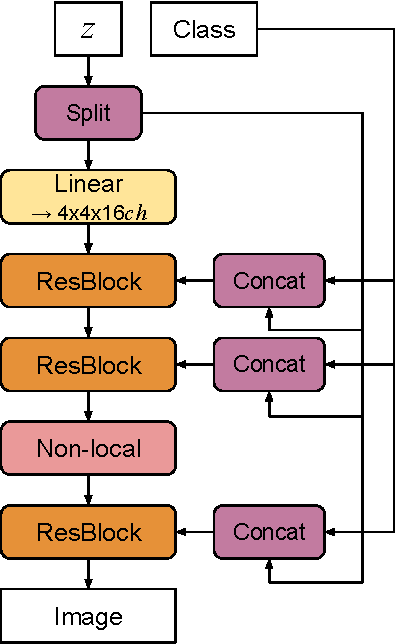
\includegraphics[width=0.25\textwidth]{images/ArchitectureMain-BigGAN.pdf}}{(a)}
\hspace{0.5cm}
\subf{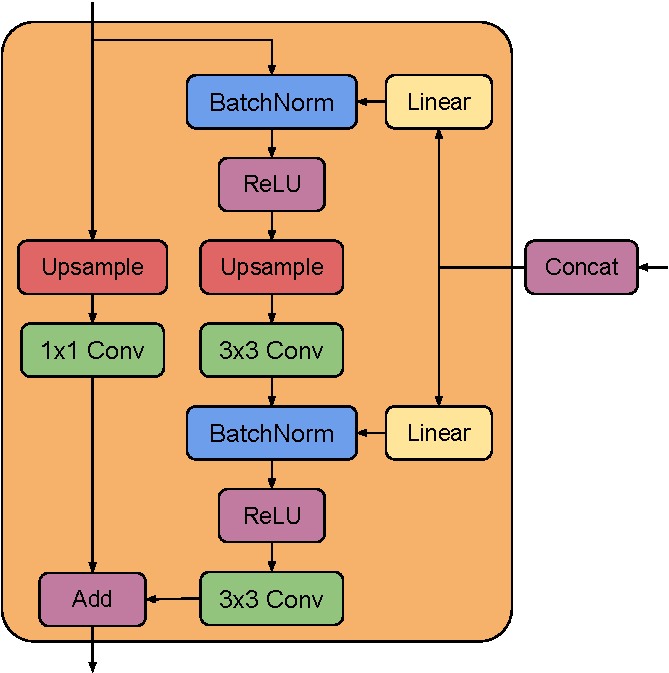
\includegraphics[width=0.38\textwidth]{images/ResBlock-BigGAN-G.pdf}}{(b)}
\hspace{0.5cm}
\subf{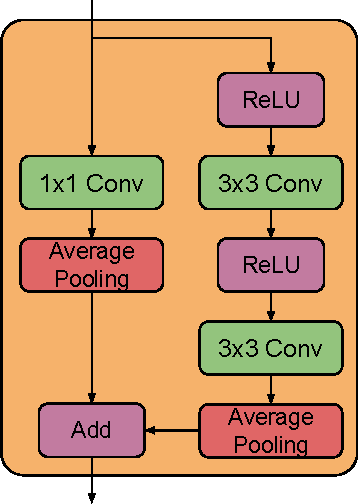
\includegraphics[width=0.2\textwidth]{images/ResBlock-BigGAN-D.pdf}}{(c)}
\end{tabular}
\caption{
(a) A typical architectural layout for BigGAN's \gen{}; details are in the following tables. 
(b) A Residual Block (\textit{ResBlock up})  in BigGAN's \gen{}.
(c) A Residual Block (\textit{ResBlock down}) in BigGAN's \discr{}.
}
\label{appendix_resblock_figure}
\end{figure}

\begin{figure}[htbp]
\centering
\begin{tabular}{c}
\subf{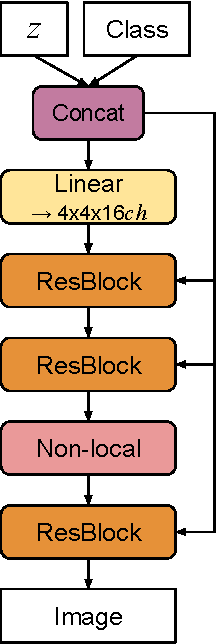
\includegraphics[width=0.15\textwidth]{images/ArchitectureMain-BigGAN-deep.pdf}}{(a)} \\
\subf{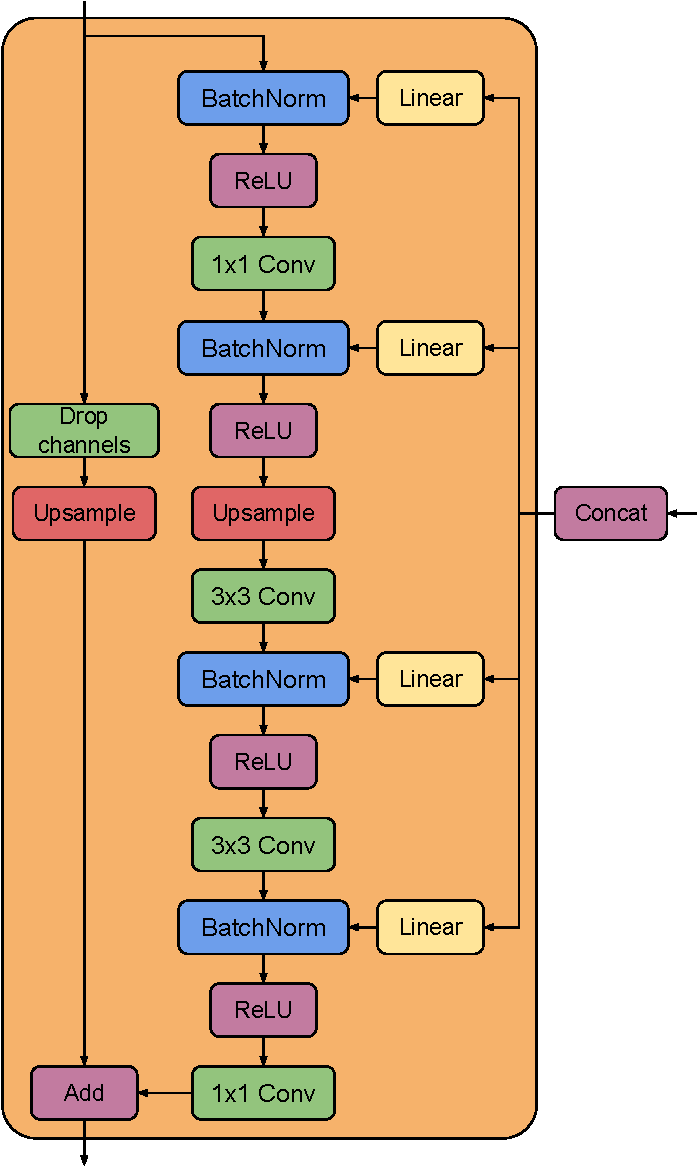
\includegraphics[width=0.45\textwidth]{images/ResBlock-BigGAN-deep-G.pdf}}{(b)}
\hspace{2cm}
\subf{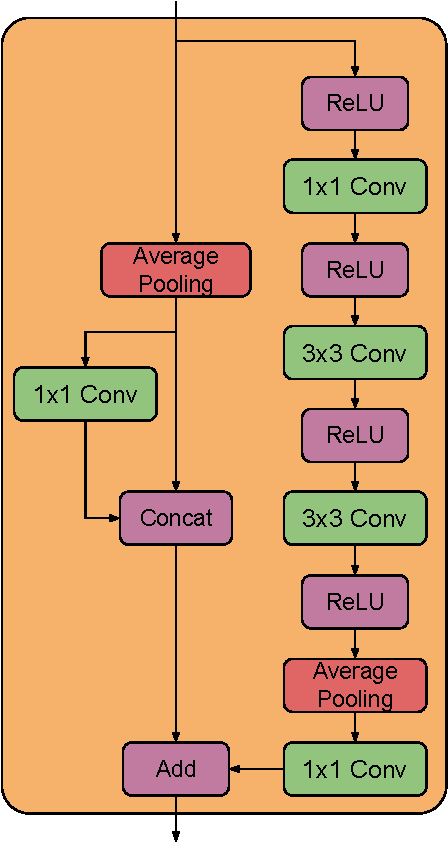
\includegraphics[width=0.3\textwidth]{images/ResBlock-BigGAN-deep-D.pdf}}{(c)}
\end{tabular}
\caption{
(a) A typical architectural layout for BigGAN-deep's \gen{}; details are in the following tables. 
(b) A Residual Block (\textit{ResBlock up}) in BigGAN-deep's \gen{}.
(c) A Residual Block (\textit{ResBlock down}) in BigGAN-deep's \discr{}.
A \textit{ResBlock} (without \textit{up} or \textit{down}) in BigGAN-deep does not include the \textit{Upsample} or \textit{Average Pooling} layers, and has identity skip connections.
}
\label{appendix_resblock_figure_deep}
\end{figure}

\begin{table}[ht]
         \caption{\label{tab:resnets_imagenet128} BigGAN architecture for $128\times 128$ images. $ch$ represents the channel width multiplier in each network from Table~\ref{ablation_table}.}
          \centering
          \small
          \begin{subtable}{.4\textwidth}
              \centering
              {\begin{tabular}{c}
                  \toprule
                  \midrule
                  $z\in \bbR^{120} \sim \mathcal{N}(0, I)$ \\
                  Embed($y$) $\in \bbR^{128}$ \\
                  \midrule
                  Linear $(20+128) \rightarrow 4 \times 4 \times 16 ch $ \\
                  \midrule
                  ResBlock up $16ch \rightarrow 16ch$ \\
                  \midrule
                  ResBlock up $16ch \rightarrow 8ch$\\
                  \midrule
                  ResBlock up $8ch \rightarrow 4ch$\\
                  \midrule
                  ResBlock up $4ch \rightarrow 2ch$\\
                  \midrule
                  Non-Local Block ($64\times 64$)\\
                  \midrule
                  ResBlock up $2ch \rightarrow ch$\\
                  \midrule
                  BN, ReLU, $3\times 3$ Conv $ch\rightarrow 3$ \\
                  \midrule
                  Tanh\\
                  \midrule
                  \bottomrule
              \end{tabular}}
              \caption{\label{tab:gen_resnet_imagenet_128} Generator}
          \end{subtable}
          \begin{subtable}{.4\textwidth}
              \centering
              {\begin{tabular}{c}
                  \toprule
                  \midrule
                  RGB image $x\in \bbR^{128 \times 128 \times 3}$ \\
                  \midrule
                  ResBlock down $ch \rightarrow 2ch$\\
                  \midrule
                  Non-Local Block ($64\times 64$) \\
                  \midrule
                  ResBlock down $2ch \rightarrow 4ch$\\
                  \midrule
                  ResBlock down $4ch \rightarrow 8ch$\\
                  \midrule
                  ResBlock down $8ch \rightarrow 16ch$\\
                  \midrule
                  ResBlock down $16ch \rightarrow 16ch$\\
                  \midrule
                  ResBlock $16ch \rightarrow 16ch$\\
                  \midrule
                  ReLU, Global sum pooling\\
                  \midrule
                  Embed($y$)$\cdot \bmh$ + (linear $\rightarrow$ 1) \\
                  \midrule
                  \bottomrule
              \end{tabular}}
              \caption{\label{tab:dis_resnet_imagenet_128} Discriminator}
          \end{subtable}
\end{table}

\begin{table}[ht]
         \caption{\label{tab:resnets_imagenet256} BigGAN architecture for $256\times 256$ images. 
         Relative to the $128\times 128$ architecture, we add an additional ResBlock in each network at 16$\times$16 resolution, and move the non-local block in \gen{} to $128\times 128$ resolution. Memory constraints prevent us from moving the non-local block in \discr{}.}
          \centering
          \small
          \begin{subtable}{.4\textwidth}
              \centering
              {\begin{tabular}{c}
                  \toprule
                  \midrule
                  $z\in \bbR^{140} \sim \mathcal{N}(0, I)$ \\
                  Embed($y$) $\in \bbR^{128}$ \\
                  \midrule
                  Linear $(20+128) \rightarrow 4 \times 4 \times 16 ch $ \\
                  \midrule
                  ResBlock up $16ch \rightarrow 16ch$ \\
                  \midrule
                  ResBlock up $16ch \rightarrow 8ch$\\
                  \midrule
                  ResBlock up $8ch \rightarrow 8ch$\\
                  \midrule
                  ResBlock up $8ch \rightarrow 4ch$\\
                  \midrule
                  ResBlock up $4ch \rightarrow 2ch$\\
                  \midrule
                  Non-Local Block ($128\times 128$) \\
                  \midrule
                  ResBlock up $2ch \rightarrow ch$\\
                  \midrule
                  BN, ReLU, $3\times 3$ Conv $ch\rightarrow 3$ \\
                  \midrule
                  Tanh\\
                  \midrule
                  \bottomrule
              \end{tabular}}
              \caption{\label{tab:gen_resnet_imagenet_256} Generator}
          \end{subtable}
          \begin{subtable}{.4\textwidth}
              \centering
              {\begin{tabular}{c}
                  \toprule
                  \midrule
                  RGB image $x\in \bbR^{256 \times 256 \times 3}$ \\
                  \midrule
                  ResBlock down $ch \rightarrow 2ch$\\
                  \midrule
                  ResBlock down $2ch \rightarrow 4ch$\\
                  \midrule
                  Non-Local Block ($64\times 64$) \\
                  \midrule
                  ResBlock down $4ch \rightarrow 8ch$\\
                  \midrule
                  ResBlock down $8ch \rightarrow 8ch$\\
                  \midrule
                  ResBlock down $8ch \rightarrow 16ch$\\
                  \midrule
                  ResBlock down $16ch \rightarrow 16ch$\\
                  \midrule
                  ResBlock $16ch \rightarrow 16ch$\\
                  \midrule
                  ReLU, Global sum pooling\\
                  \midrule
                  Embed($y$)$\cdot \bmh$ + (linear $\rightarrow$ 1) \\
                  \midrule
                  \bottomrule
              \end{tabular}}
              \caption{\label{tab:dis_resnet_imagenet_256} Discriminator}
          \end{subtable}
\end{table}

\begin{table}[ht]
         \caption{\label{tab:resnets_imagenet512} BigGAN architecture for $512\times 512$ images.
         Relative to the $256\times 256$ architecture, we add an additional ResBlock at the $512\times 512$ resolution. Memory constraints force us to move the non-local block in both networks back to  $64\times 64$ resolution as in the $128\times 128$ pixel setting.}
          \centering
          \small
          \begin{subtable}{.4\textwidth}
              \centering
              {\begin{tabular}{c}
                  \toprule
                  \midrule
                  $z\in \bbR^{160} \sim \mathcal{N}(0, I)$ \\
                  Embed($y$) $\in \bbR^{128}$ \\
                  \midrule
                  Linear $(20+128) \rightarrow 4 \times 4 \times 16 ch $ \\
                  \midrule
                  ResBlock up $16ch \rightarrow 16ch$ \\
                  \midrule
                  ResBlock up $16ch \rightarrow 8ch$\\
                  \midrule
                  ResBlock up $8ch \rightarrow 8ch$\\
                  \midrule
                  ResBlock up $8ch \rightarrow 4ch$\\
                   \midrule
                  Non-Local Block ($64\times 64$) \\
                  \midrule
                  ResBlock up $4ch \rightarrow 2ch$\\
                 \midrule
                  ResBlock up $2ch \rightarrow ch$\\
                  \midrule
                  ResBlock up $ch \rightarrow ch$\\
                  \midrule
                  BN, ReLU, $3\times 3$ Conv $ch\rightarrow 3$ \\
                  \midrule
                  Tanh\\
                  \midrule
                  \bottomrule
              \end{tabular}}
              \caption{\label{tab:gen_resnet_imagenet_512} Generator}
          \end{subtable}
          \begin{subtable}{.4\textwidth}
              \centering
              {\begin{tabular}{c}
                  \toprule
                  \midrule
                  RGB image $x\in \bbR^{512 \times 512 \times 3}$ \\
                  \midrule
                  ResBlock down $ch \rightarrow ch$\\
                  \midrule
                  ResBlock down $ch \rightarrow 2ch$\\
                  \midrule
                  ResBlock down $2ch \rightarrow 4ch$\\
                  \midrule
                  Non-Local Block ($64\times 64$) \\
                  \midrule
                  ResBlock down $4ch \rightarrow 8ch$\\
                  \midrule
                  ResBlock down $8ch \rightarrow 8ch$\\
                  \midrule
                  ResBlock down $8ch \rightarrow 16ch$\\
                  \midrule
                  ResBlock down $16ch \rightarrow 16ch$\\
                  \midrule
                  ResBlock $16ch \rightarrow 16ch$\\
                  \midrule
                  ReLU, Global sum pooling\\
                  \midrule
                  Embed($y$)$\cdot \bmh$ + (linear $\rightarrow$ 1) \\
                  \midrule
                  \bottomrule
              \end{tabular}}
              \caption{\label{tab:dis_resnet_imagenet_512} Discriminator}
          \end{subtable}
\end{table}

\begin{table}[ht]
         \caption{\label{tab:deep_resnets_imagenet128} BigGAN-deep architecture for $128\times 128$ images.}
          \centering
          \small
          \begin{subtable}{.4\textwidth}
              \centering
              {\begin{tabular}{c}
                  \toprule
                  \midrule
                  $z\in \bbR^{128} \sim \mathcal{N}(0, I)$ \\
                  Embed($y$) $\in \bbR^{128}$ \\
                  \midrule
                  Linear $(128+128) \rightarrow 4 \times 4 \times 16 ch $ \\
                  \midrule
                  ResBlock $16ch \rightarrow 16ch$ \\
                  \midrule
                  ResBlock up $16ch \rightarrow 16ch$ \\
                  \midrule
                  ResBlock $16ch \rightarrow 16ch$ \\
                  \midrule
                  ResBlock up $16ch \rightarrow 8ch$ \\
                  \midrule
                  ResBlock $8ch \rightarrow 8ch$ \\
                  \midrule
                  ResBlock up $8ch \rightarrow 4ch$ \\
                  \midrule
                  ResBlock $4ch \rightarrow 4ch$ \\
                  \midrule
                  ResBlock up $4ch \rightarrow 2ch$ \\
                  \midrule
                  Non-Local Block ($64\times 64$)\\
                  \midrule
                  ResBlock $2ch \rightarrow 2ch$ \\
                  \midrule
                  ResBlock up $2ch \rightarrow ch$ \\
                  \midrule
                  BN, ReLU, $3\times 3$ Conv $ch\rightarrow 3$ \\
                  \midrule
                  Tanh\\
                  \midrule
                  \bottomrule
              \end{tabular}}
              \caption{\label{tab:deep_gen_resnet_imagenet_128} Generator}
          \end{subtable}
          \begin{subtable}{.4\textwidth}
              \centering
              {\begin{tabular}{c}
                  \toprule
                  \midrule
                  RGB image $x\in \bbR^{128 \times 128 \times 3}$ \\
                  \midrule
                  $3\times 3$ Conv $3\rightarrow ch$\\
                  \midrule
                  ResBlock down $ch \rightarrow 2ch$\\
                  \midrule
                  ResBlock $2ch \rightarrow 2ch$\\
                  \midrule
                  Non-Local Block ($64\times 64$) \\
                  \midrule
                  ResBlock down $2ch \rightarrow 4ch$\\
                  \midrule
                  ResBlock $4ch \rightarrow 4ch$\\
                  \midrule
                  ResBlock down $4ch \rightarrow 8ch$\\
                  \midrule
                  ResBlock $8ch \rightarrow 8ch$\\
                  \midrule
                  ResBlock down $8ch \rightarrow 16ch$\\
                  \midrule
                  ResBlock $16ch \rightarrow 16ch$\\
                  \midrule
                  ResBlock down $16ch \rightarrow 16ch$\\
                  \midrule
                  ResBlock $16ch \rightarrow 16ch$\\
                  \midrule
                  ReLU, Global sum pooling\\
                  \midrule
                  Embed($y$)$\cdot \bmh$ + (linear $\rightarrow$ 1) \\
                  \midrule
                  \bottomrule
              \end{tabular}}
              \caption{\label{tab:deep_dis_resnet_imagenet_128} Discriminator}
          \end{subtable}
\end{table}

\begin{table}[ht]
         \caption{\label{tab:deep_resnets_imagenet256} BigGAN-deep architecture for $256\times 256$ images.}
          \centering
          \small
          \begin{subtable}{.4\textwidth}
              \centering
              {\begin{tabular}{c}
                  \toprule
                  \midrule
                  $z\in \bbR^{128} \sim \mathcal{N}(0, I)$ \\
                  Embed($y$) $\in \bbR^{128}$ \\
                  \midrule
                  Linear $(128+128) \rightarrow 4 \times 4 \times 16 ch $ \\
                  \midrule
                  ResBlock $16ch \rightarrow 16ch$ \\
                  \midrule
                  ResBlock up $16ch \rightarrow 16ch$ \\
                  \midrule
                  ResBlock $16ch \rightarrow 16ch$ \\
                  \midrule
                  ResBlock up $16ch \rightarrow 8ch$ \\
                  \midrule
                  ResBlock $8ch \rightarrow 8ch$ \\
                  \midrule
                  ResBlock up $8ch \rightarrow 8ch$ \\
                  \midrule
                  ResBlock $8ch \rightarrow 8ch$ \\
                  \midrule
                  ResBlock up $8ch \rightarrow 4ch$ \\
                  \midrule
                  Non-Local Block ($64\times 64$)\\
                  \midrule
                  ResBlock $4ch \rightarrow 4ch$ \\
                  \midrule
                  ResBlock up $4ch \rightarrow 2ch$ \\
                  \midrule
                  ResBlock $2ch \rightarrow 2ch$ \\
                  \midrule
                  ResBlock up $2ch \rightarrow ch$ \\
                  \midrule
                  BN, ReLU, $3\times 3$ Conv $ch\rightarrow 3$ \\
                  \midrule
                  Tanh\\
                  \midrule
                  \bottomrule
              \end{tabular}}
              \caption{\label{tab:deep_gen_resnet_imagenet_256} Generator}
          \end{subtable}
          \begin{subtable}{.4\textwidth}
              \centering
              {\begin{tabular}{c}
                  \toprule
                  \midrule
                  RGB image $x\in \bbR^{256 \times 256 \times 3}$ \\
                  \midrule
                  $3\times 3$ Conv $3\rightarrow ch$\\
                  \midrule
                  ResBlock down $ch \rightarrow 2ch$\\
                  \midrule
                  ResBlock $2ch \rightarrow 2ch$\\
                  \midrule
                  ResBlock down $2ch \rightarrow 4ch$\\
                  \midrule
                  ResBlock $4ch \rightarrow 4ch$\\
                  \midrule
                  Non-Local Block ($64\times 64$) \\
                  \midrule
                  ResBlock down $4ch \rightarrow 8ch$\\
                  \midrule
                  ResBlock $8ch \rightarrow 8ch$\\
                  \midrule
                  ResBlock down $8ch \rightarrow 8ch$\\
                  \midrule
                  ResBlock $8ch \rightarrow 8ch$\\
                  \midrule
                  ResBlock down $8ch \rightarrow 16ch$\\
                  \midrule
                  ResBlock $16ch \rightarrow 16ch$\\
                  \midrule
                  ResBlock down $16ch \rightarrow 16ch$\\
                  \midrule
                  ResBlock $16ch \rightarrow 16ch$\\
                  \midrule
                  ReLU, Global sum pooling\\
                  \midrule
                  Embed($y$)$\cdot \bmh$ + (linear $\rightarrow$ 1) \\
                  \midrule
                  \bottomrule
              \end{tabular}}
              \caption{\label{tab:deep_dis_resnet_imagenet_256} Discriminator}
          \end{subtable}
\end{table}

\begin{table}[ht]
         \caption{\label{tab:deep_resnets_imagenet512} BigGAN-deep architecture for $512\times 512$ images.}
          \centering
          \small
          \begin{subtable}{.4\textwidth}
              \centering
              {\begin{tabular}{c}
                  \toprule
                  \midrule
                  $z\in \bbR^{128} \sim \mathcal{N}(0, I)$ \\
                  Embed($y$) $\in \bbR^{128}$ \\
                  \midrule
                  Linear $(128+128) \rightarrow 4 \times 4 \times 16 ch $ \\
                  \midrule
                  ResBlock $16ch \rightarrow 16ch$ \\
                  \midrule
                  ResBlock up $16ch \rightarrow 16ch$ \\
                  \midrule
                  ResBlock $16ch \rightarrow 16ch$ \\
                  \midrule
                  ResBlock up $16ch \rightarrow 8ch$ \\
                  \midrule
                  ResBlock $8ch \rightarrow 8ch$ \\
                  \midrule
                  ResBlock up $8ch \rightarrow 8ch$ \\
                  \midrule
                  ResBlock $8ch \rightarrow 8ch$ \\
                  \midrule
                  ResBlock up $8ch \rightarrow 4ch$ \\
                  \midrule
                  Non-Local Block ($64\times 64$)\\
                  \midrule
                  ResBlock $4ch \rightarrow 4ch$ \\
                  \midrule
                  ResBlock up $4ch \rightarrow 2ch$ \\
                  \midrule
                  ResBlock $2ch \rightarrow 2ch$ \\
                  \midrule
                  ResBlock up $2ch \rightarrow ch$ \\
                  \midrule
                  ResBlock $ch \rightarrow ch$ \\
                  \midrule
                  ResBlock up $ch \rightarrow ch$ \\
                  \midrule
                  BN, ReLU, $3\times 3$ Conv $ch\rightarrow 3$ \\
                  \midrule
                  Tanh\\
                  \midrule
                  \bottomrule
              \end{tabular}}
              \caption{\label{tab:deep_gen_resnet_imagenet_512} Generator}
          \end{subtable}
          \begin{subtable}{.4\textwidth}
              \centering
              {\begin{tabular}{c}
                  \toprule
                  \midrule
                  RGB image $x\in \bbR^{512 \times 512 \times 3}$ \\
                  \midrule
                  $3\times 3$ Conv $3\rightarrow ch$\\
                  \midrule
                  ResBlock down $ch \rightarrow ch$\\
                  \midrule
                  ResBlock $ch \rightarrow ch$\\
                  \midrule
                  ResBlock down $ch \rightarrow 2ch$\\
                  \midrule
                  ResBlock $2ch \rightarrow 2ch$\\
                  \midrule
                  ResBlock down $2ch \rightarrow 4ch$\\
                  \midrule
                  ResBlock $4ch \rightarrow 4ch$\\
                  \midrule
                  Non-Local Block ($64\times 64$) \\
                  \midrule
                  ResBlock down $4ch \rightarrow 8ch$\\
                  \midrule
                  ResBlock $8ch \rightarrow 8ch$\\
                  \midrule
                  ResBlock down $8ch \rightarrow 8ch$\\
                  \midrule
                  ResBlock $8ch \rightarrow 8ch$\\
                  \midrule
                  ResBlock down $8ch \rightarrow 16ch$\\
                  \midrule
                  ResBlock $16ch \rightarrow 16ch$\\
                  \midrule
                  ResBlock down $16ch \rightarrow 16ch$\\
                  \midrule
                  ResBlock $16ch \rightarrow 16ch$\\
                  \midrule
                  ReLU, Global sum pooling\\
                  \midrule
                  Embed($y$)$\cdot \bmh$ + (linear $\rightarrow$ 1) \\
                  \midrule
                  \bottomrule
              \end{tabular}}
              \caption{\label{tab:deep_dis_resnet_imagenet_512} Discriminator}
          \end{subtable}
\end{table}


\clearpage